\documentclass[a4paper, 11pt, notitlepage]{article}
\addtolength{\hoffset}{-1cm}
\addtolength{\textwidth}{2cm}
\usepackage[utf8]{inputenc}
\usepackage[frenchb]{babel}
\usepackage[T1]{fontenc}

\usepackage{multicol}
\usepackage{listings}
\usepackage{graphicx}
\usepackage{hyperref}
\usepackage{amssymb}
\usepackage{amsmath}

\usepackage{color}
\definecolor{lightgray}{rgb}{.9,.9,.9}
\definecolor{darkgray}{rgb}{.5,.2,.2}
\definecolor{purple}{rgb}{0.65, 0.12, 0.82}
\definecolor{brown}{RGB}{140, 0, 0}

\lstnewenvironment{OCaml}
                  {\lstset{
                      language=[Objective]Caml,
                      breaklines=true,
                      showstringspaces=false,
                      commentstyle=\color{red},
                      stringstyle=\color{darkgray},
                      identifierstyle=\ttfamily,
                      keywordstyle=\color{blue},
                      basicstyle=\footnotesize,
                      escapeinside={/*}{*/},
                      %xleftmargin=0.08\textwidth
                    }
                  }
                  {}
\lstnewenvironment{OCamlEx}
                  {\lstset{
                      language=[Objective]Caml,
                      breaklines=true,
                      showstringspaces=false,
                      commentstyle=\color{red},
                      stringstyle=\color{darkgray},
                      identifierstyle=\ttfamily,
                      keywordstyle=\color{blue},
                      basicstyle=\footnotesize,
                     escapeinside={/*}{*/},
                      frame=single,
                      numbers=left,
                      %xleftmargin=0.08\textwidth
                    }
                  }
                  {}
\newcommand{\class}{\ttfamily\textit{class}}
\newcommand{\interface}{\ttfamily\textit{interface}}
\newcommand{\name}{\ttfamily\textit{name}}
\newcommand{\package}{\ttfamily\textit{package}}
\newcommand{\ident}{\footnotesize\textbf{ident}}
\newcommand{\fun}[1]{\ttfamily\textbf{#1}}

\lstdefinelanguage{idlgrammar}{
  morekeywords={package,abstract,extends,class,implements,static,final,<ini>,interface,callback,array,[,],{,},
    name ,void,boolean,byte,char,short,int,long,float,double,string},
  alsoletter=[]{},
}
\lstnewenvironment{idl}
                  {\lstset{
                      language=idlgrammar,
                      breaklines=true,
                      showstringspaces=false,
                      keywordstyle=\ttfamily\color{blue},
                      identifierstyle=\ttfamily\textit,
                      basicstyle=\footnotesize,
                     escapeinside={(*}{*)},
                      %xleftmargin=0.08\textwidth
                    }
                  }
                  {} 
\lstnewenvironment{idlEx}
                  {\lstset{
                      language=idlgrammar,
                      breaklines=true,
                      showstringspaces=false,
                      commentstyle=\color{red},
                      stringstyle=\color{darkgray},
                      identifierstyle=\ttfamily\textit,
                      keywordstyle=\color{blue},
                      basicstyle=\footnotesize,
                     escapeinside={/*}{*/},
                      frame=single,
                      numbers=left,
                      %xleftmargin=0.08\textwidth
                    }
                  }
                  {}


%%%%%%%%%%%%%%%%%%%%%%%%%%%%%%%%%%%%%%%%%%%%%%%%%%%%%%%%%%%%%%%%%%%%%%%%%%%%%%



\title{
  \huge L'interopérabilité entre OCaml et Java\\
}
\author{
  Béatrice Carré \\
  beatrice.carre@etu.upmc.fr \\
  \\
  Encadrants : Emmanuel Chailloux, Xavier Clerc et Grégoire Henry \\
}

\begin{document}
\maketitle
\tableofcontents
\newpage

\section*{Introduction}
\addcontentsline{toc}{section}{Introduction}
Il est parfois utile de réutiliser des structures
écrites dans un certain langage sans avoir à les réécrire entièrement.
Il peut arriver de vouloir utiliser l'efficacité et
l'élégance du style fonctionnel d'Ocaml dans un
programme autant que la portabilité du style objet de Java et la
diversité de son API.

C'est pourquoi l'interopérabilité est un problème intéressant.
Mais elle engendre beaucoup de questions sur la gestion de
plusieurs éléments :
la cohérence des types d'un langage à l'autre,
la copie ou le partage des valeurs d'un monde à l'autre,
le passage des exceptions,
la gestion automatique de la mémoire (GC), 
et des caractéristiques de programmation qui ne sont pas forcément gérées par les
deux langages.

OCaml et Java comportent des différences entre leur modèles
objet, comme le montre le tableau ci-dessous, il donc est nécessaire
de réduire l'étude à leur l'intersection.

\ 
\newline
\noindent
\begin{tabular}{|l|c|c|c|c|}
  \hline
  \emph{caractéristiques} & \emph{Java} & \emph{OCaml} \\
  \hline
  accès champs & selon la visibilité & via appels de méthode\\\hline
  variables/méthodes statiques & \checkmark & fonctions/décl. globales\\\hline
  typage dynamique & \checkmark & pas de downcast \\\hline
  héritage $\equiv$ sous-typage ? &\checkmark  & $\times$ \\\hline
  surcharge & \checkmark & $\times$ \\\hline
  héritage multiple & seulement pour les interfaces & \checkmark\\
  \hline
  packetages/modules & pas de modules paramétrés & \checkmark\\\hline
\end{tabular}

Deux études ont déjà été réalisées pour l’interopérabilité entre
Ocaml et Java à travers leur modèle object respectif :

\emph{O’Jacaré (et Camljava)} conserve les runtimes des deux langages (GC,
Exceptions, ...) et les fait communiquer par l'interface camljava,
avec l'aide de classes encapsulantes générées par O'Jacaré.

\emph{OCaml-java
  2.0} utilise un seul runtime, en compilant le OCaml en byte-code
Java. La manipulation des classes Java se fait à l'aide de nouveaux types introduits.
\newline

L'idée est de profiter des deux approches : d'une part, d'un accès simple à des classes
définies, en générant le code nécessaire à cet accès grâce à O'Jacaré
et d'autre part de l'accès direct à toute
l'API Java en ne gardant qu'un seul runtime, la
JRE, grâce à OCaml-Java

Après l’étude des deux outils, le projet consiste à engendrer pour
ocaml-java les fichiers d’encapsulation d'O’Jacaré. Ce
portage est réalisé en OCaml étant donné qu'il reprend ce qui
a déjà été développé pour O’Jacaré. Cette adaptation ne gère pas les appels de Java vers OCaml (callback), ainsi que les tableaux.
\newline

Dans ce rapport, nous décrivons le schéma global du
générateur de code d'O'Jacaré, et celui du compilateur d'Ocaml-Java
pour en faire ressortir les avantages d'un portage d'O'Jacaré pour OCaml-Java.
Nous détaillons par la suite les modifications apportées à la
génération d'interfaces, adaptée pour une encapsulation utilisable par
le compilateur d'OCaml-Java.
Pour finir, un exemple d'application vous sera présenté.
\newpage









\section{L'interopérabilité entre OCaml et Java}

%%%%%%%%%%%%%%%%%%%%%%%%%%%%%%%%%  1.1  O'Jacaré   %%%%%%%%%%%%%%%%%%%%%%%%%%%%%%%%%%%

\subsection{O'Jacaré, un générateur de code d'interface}

\subsubsection{Principe global}
O'Jacaré génère le code nécessaire à l'encapsulation des classes
définies dans un IDL, pour permettre aux interfaces avec C de chacunes
de communiquer.

L'appel à des classes et méthodes Java est alors possible en appelant
les méthodes de la capsule générée, qui va gérer l'appel aux classes
Java par le biais de l'interface camlJava.
Les stubs générés par le callback vont permettre avec le même
principe, les appels dans l'autre sens.

CamlJava est une interface bas-niveau basée sur les interfaces de chaque langage avec C : la JNI (Java Native Interface) et external.

La génération de code se fait en plusieurs passes :
\begin{itemize}
\item analyse lexicale et analyse syntaxique de l' idl donnant un AST.
\item vérification des types de l'AST, donnant un nouvel arbre CAST.
\item la génération des fichiers stub java nécessaires pour un appel callback. 
\item la génération à partir du CAST des classes encapsulantes dans un fichier .ml
\item la génération à partir du CAST du module .mli adapté
\end{itemize}
Les deux dernières étapes seront présentées plus en profondeur dans la
section TODO.
Un schéma décrit ces étapes dans la figure 2.

\begin{figure}[h]
  \centering
  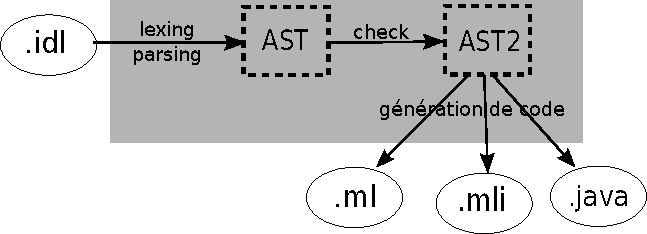
\includegraphics{schemaOjacare.pdf}
  \caption{Schéma global de la génération d'O'Jacaré}
\end{figure}

\newpage

\subsubsection{la génération de code}
La génération de code se fait à partir d'un IDL, dont la grammaire
(BNF) est définie en annexe.
Dans cet IDL, nous pouvons définir des déclarations qui sont à
l'intersection de ce qui est accessible dans les modèles objet de
chaque langage. 

Le but de cet IDL est de définir la signature des
classes Java déjà définies, que nous voulons manipuler du côté OCaml.
Ces classes encapsulantes servant à faire le liens entre les
classes/interfaces de chaque côté, il n'est donc nécessaire de définir
dans l'IDL uniquement les méthodes que nous voulons appeler depuis OCaml.

Voici un exemple de déclarations pour la fameuse classe Point dans un
fichier IDL.

\begin{idlEx}
package mypack;
class Point {
  int x;
  int y; 
  [name default_point] <init> ();
  [name point] <init> (int,int);
  void moveto(int,int);
  string toString();
  boolean eq(Point);
}
interface Colored {
  string getColor();
  void setColor(string);
}
class ColoredPoint extends Point implements Colored {
  [name default_colored_point] <init> ();
  [name colored_point] <init> (int,int,string);
  [name eq_colored_point] boolean eq(ColoredPoint);
}
\end{idlEx}

Pour une déclaration de classe ou interface, la génération de code
donne :
\begin{itemize}
  \item Un type objet t
  \item Une classe encapsulante C de type t
  \item 1 à n classes Ci, sous-classes de C (une par constructeur),
 
    0 si c'est une interface
  \item Une fonction instanceof pour ce type
  \item Une fonction de cast pour ce type
\end{itemize}

Les fichiers générés sont destinés à être compilés avec l'aide la bibliothèque
Camljava.

\newpage
\subsubsection{compilation par camljava}
Camljava gère l'interfacage entre OCaml et Java avec C, comme décrit
dans la figure 3.
Les références sur les objets Java correspondent à un type abstrait en
OCaml, sur lesquels des opérations donnent accès à des méthodes, à des
champs ou autres. 

L'exécution se fait dans les 2 runtimes, qui peuvent alors communiquer.

La gestion des exceptions est faite par encapsulation aussi, et la
gestion de la mémoire se fait par une mise en racine de l'objet dans
l'autre monde avant de le passer en référence.

\begin{figure}[h]
  \centering
  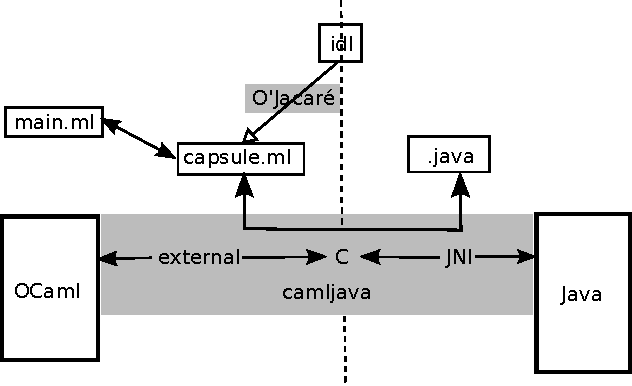
\includegraphics{schemaCamljava2.pdf}
  \caption{La communication grâce à Camljava}
\end{figure}









%%%%%%%%%%%%%%%%%%%%%%%%%%%%%%%%%  1.2  OCaml-Java   %%%%%%%%%%%%%%%%%%%%%%%%%%%%%%%%%%%

\subsection{OCaml-Java et la compilation de code OCaml vers du bytecode Java}

\subsubsection{Principe Global}
intro TODO presentation OCaml-Java



\begin{figure}[h]
  \centering
  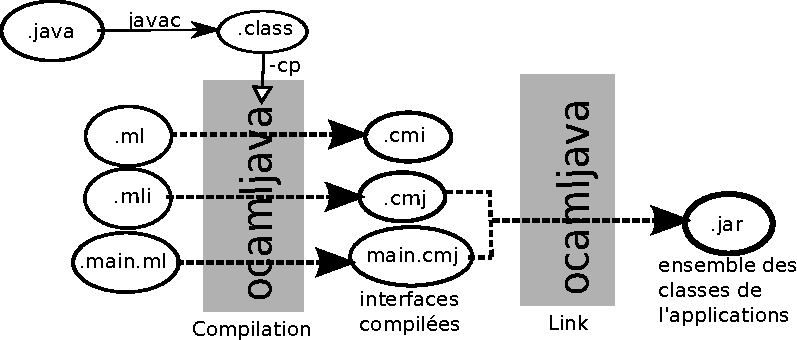
\includegraphics{schemaOCamlJava.pdf}
  \caption{Schéma global du compilateur d'OCaml-Java}
\end{figure}

\subsubsection{Accès à du code Java}
\noindent
Description des types manipulés par OCaml-Java permettant un accès au
monde de Java depuis celui d'OCaml.  

\begin{tabular}{|l|l|}
  \hline
  type Java & description et exemple \\
  \hline
  java\_constructor & signature d'un constructeur  \\
  &  "java.lang.Object()" \\
  \hline
  java\_method & signature d'une méthode \\
  & "java.lang.String.lastIndexOf(string):int"\\
  \hline
  java\_field\_get & signature d'un attribut\\
  & "mypack.Point.x:int" \\
  \hline
  java\_field\_set & signature d'un attribut\\
  & "mypack.Point.x:int" \\
  \hline
  java\_type & classe, interface ou type Array\\
  & "java.lang.String"\\
  \hline
  java\_proxy & type d'une interface\\
  & "java.lang.Comparable"\\ 
  \hline
\end{tabular}

\noindent
Description du module Java

\begin{OCamlEx}
make : 'a java_constructor -> 'a 
call : 'a java_method -> 'a 
get : 'a java_field_get -> 'a 
set : 'a java_field_set -> 'a 
is_null : 'a java_instance -> bool 
instanceof : 'a java_type -> 'b java_instance -> bool
cast : 'a java_type -> 'b java_instance -> 'a
proxy : 'a java_proxy -> 'a
\end{OCamlEx}
Une exception est définie dans le module pour permettre d'attraper les
exceptions du côté OCaml :
\begin{OCamlEx}
exception Java_exception of java'lang'Throwable java_instance
\end{OCamlEx}
\newpage
Exemple :
\begin{OCamlEx}
let color = JavaString.of_string "bleu"
and x = Int32.of_int 1
and y = Int32.of_int 2 in
let p = Java.make "mypack.ColoredPoint(int,int,java.lang.String)" s y color 
in
   Java.call "mypack.Point.eq(mypack.Point):boolean" p p2
\end{OCamlEx}





\begin{OCamlEx}
let _init_point =
  let clazz = Jni.find_class "mypack/Point" in
  let id =
    try Jni.get_methodID clazz "<init>" "(II)V"
    with
    | _ ->
        failwith
          "Unknown constructor from IDL in class \"mypack.Point\" : \"Point(int,int)\"."
  in
    fun (java_obj : _jni_jPoint) _p0 _p1 ->
      let _p1 = _p1 in
      let _p0 = _p0
      in
        Jni.call_nonvirtual_void_method java_obj clazz id
          [| Jni.Camlint _p0; Jni.Camlint _p1 |];;
class point _p0 _p1 =
  let java_obj = _alloc_jPoint ()
  in let _ = _init_point java_obj _p0 _p1
    in object (self) inherit _capsule_jPoint java_obj end;;
\end{OCamlEx}
\begin{OCamlEx}
class point _p0 _p1 =
  let _p1 = Int32.of_int _p1
  in let _p0 = Int32.of_int _p0
    in let java_obj = Java.make "mypack.Point(int,int)" _p0 _p1
      in object (self) inherit _capsule_jPoint java_obj end;;
\end{OCamlEx}



%%%%%%%%%%%%%%%%%%%%%%%%%%%%  1.3  PROBLEME, IDEE de solution   %%%%%%%%%%%%%%%%%%%%%%%%%%%%%%

\subsection{profiter des deux approches}
O'Jacaré construit les classes encapsulantes de classes
java définies par l'utilisateur, et permet ainsi l'accès aux méthodes
(d'instance ou de classe) Java en OCaml en passant par l'interface de bas niveau CamlJava.
Cette interface de bas-niveau 

OCaml-Java permet l'accès à toute l'API Java depuis OCaml TODO

\ 
\newline
Solution problèmes : TODO
- gestion de la surchage (absente en OCaml) -> renommage obligatoire
dans IDL.
- 2 runtimes vs 1 seul (-> résoud pd de communication GC et exceptions)
- gestion du typage (statype en OCaml vs dynamique en Java)
-

sortie prématurée du sensé binome -> manque de temps.
Restriction : pas CB, pas gestion array.

\subsection{travail à effectuer}

étude outils O'Jacaré, mais aussi fonctionnement Camljava pour pouvoir
comparer avec cible du fichier généré : OCamljava à) la place.






%%%%%%%%%%%%%%%%%%%%%%%%%%%%  2  REALISATION   %%%%%%%%%%%%%%%%%%%%%%%%%%%%%%

\section{Portage d'O'Jacaré pour OCaml-Java}


\subsection{La génération d'O'Jacaré}
\subsubsection{La syntaxe de l'idl}
L'IDL est défini pour la construction des interfaces entreO'Caml et
Java, il est donc défini en s'approchant de l'intersection des deux
mondes objet ( TODO : A completer : definir cette intersection )

La syntaxe du langage d'interface est donné en annexe, en utilisant la
notation BNF.

Les symboles < et > encadrent des règles optionnelles,
les terminaux sont en bleu, et les non-terminaux sont en italique.


\subsubsection{Analyse lexical, syntaxique et sémantique}
La première phase est celle d'analyse lexicale et syntaxique,
séparant l'idl en lexèmes et construisant l'AST, défini en annexe par Idl.file,
dont la structure est définie en annexe.

Vient ensuite la phase d'analyse sémantique, analysant l'AST obtenue par la
phase précédente, vérifiant si le programme est correct, et

construisant une liste de CIdl.clazz, restructurant chaque classe ou interface définie dans l'idl. 
Le module Cidl définit le nouvel AST nommé CAST allant être manipulé dans les passes de
génération de code. Il est décrit en annexe.

\subsubsection{génération stub\_file}
pour callback : génération java

\subsubsection{génération des classes encapsulantes}

Type jni

Class type

Cast JNI (up et down)

Fonction d'allocation

Capsule / souche

Downcast utilisateur (
\_downcast,
\_instance\_of)

Tableaux

Fonction d'initialisation
Classe de construction

fonctions / methodes static




\subsection{schémas de compilation actuels d'O'Jacaré}




\noindent
\begin{tabular}{|l|c|c|c|c|}
  \hline
  TYPE & jni\_type & getJni \\
  \hline
  void & & \\
  boolean & Jni.Boolean &   \\
  byte & Jni.Byte & \\
  char & Jni.Char &  \\
  short & Jni.Short &  \\
  int & Jni.Camlint &  \\
  long & Jni.Long  & \\
  float & Jni.Float & \\
  double & Jni.Double  &  \\
  string & Jni.Obj \_pi & Jni.string\_to\_java \_pi  \\
  pack/Obj& Jni.Obj \_pi & \_pi\#\_get\_jni\_jname  \\
  \hline
\end{tabular}
 














%%%%%%%%%%%%%%%%%%%%%%%%%%%%   newOjacare   %%%%%%%%%%%%%%%%%%%%%%%%%%%%%%
\subsection{Génération de code pour Ocaml-Java}

\noindent
Nous considérons un environnement contenant les  variables suivantes, initialisées à leur valuer par défaut: 

$\rho$ = "" : le nom du \textbf{package} où trouver les classes définies.

$\Lambda$ = "" : le \textbf{nom de la classe} courant.

$\gamma$ = false : si la déclaration est une \textbf{interface}.

$\theta$ = false : si l'élément porte l'attribut \textbf{callback}.

$\alpha$ = false : si l'élément est déclaré \textbf{abstract}.

$\delta$ = "JniHierarchy.top" : la classe dont \textbf{extends} la classe courante.

$\Delta$ = [] : les interfaces qu'\textbf{implements} la classe courante.
\ %%   \rho,\Lambda,\gamma,\theta,\alpha,\delta,\Delta



Tableau représentant les équivalents en OCaml des types Java manipulés
par OCaml-Java.
La troisième colonne représente les types manipulés par les programmes
OCaml écrit par l'utilisateur du nouvel outil.
Le problème est donc de convertir du deuxième au troisième type pour la manipulation côté OCaml et du troisième au second lors d'un appel à une fonction du module Java (un appel, un constructeur ou autre).

\begin{tabular}{|c|l|l|l|}
 \hline
TYPE IDL &type Java & type OCaml  pour OCaml-Java & type OCaml \\
& (java\_type) & (oj\_type t) & (ml\_type t) \\
 \hline
\emph{void} & void & unit & unit\\
\emph{boolean} &boolean & bool & bool\\
\emph{byte} & byte & int & int \\
\emph{char} &char & int & char\\
\emph{double} & double & float & float\\
\emph{float} & float & float & float\\
\emph{int} & int & int32 & int\\
\emph{long} & long & int64 & int\\
\emph{short} & short & int & int\\
\emph{string} & java.lang.String & java'lang'String java\_instance & string\\
\emph{pack/Obj} & pack.Obj & pack'Obj java\_instance & jObj\\
 \hline
\end{tabular}
\
\newline

Tableau associant pour chaque types de l'IDL les
fonctions utiles aux schémas de compilation manipulant ceux-ci, comme explicité ci-dessus. 

\begin{tabular}{|c|l|l|l|}
  \hline

  TYPE IDL & to\_oj\_Type ARGi & to\_ml\_type ARGi & fcast\\

  \hline
  \emph{void} &   &  & \\

  \emph{boolean} &  &  &\_pi \\

 \emph{byte} & &  &\_pi  \\

 \emph{cha}r & TODO  & TODO & \_pi \\

  \emph{short} & &  & \\

 \emph{int} & Int32.of\_int\ & Int32.to\_int & \_pi\\

 \emph{long} & Int64.of\_int & Int64.to\_int & \_pi\\

 \emph{float} & & &\_pi \\

  \emph{doubl}e & & & \_pi\\

 \emph{string} & JavaString.of\_string & JavaString.to\_string & \_pi\\

 \emph{pack/Obj} & \_pi\#\_get\_jni\_jObj & (new \_capsule\_jObj ... : jObj) & (\_pi: jObj)\\

  \hline
\end{tabular}

 
Le type top manipulé sera le type d'instance objet de Ocaml-Java :
\begin{OCamlEx}
type top = java'lang'Object java_instance;;
\end{OCamlEx}

Exception :
\begin{OCamlEx}
exception Null_object of string
\end{OCamlEx}




\ 
\newline
\textbf{class}

Le schéma de compilation de base pour une classe est largement allégé. 
En effet,la fonction downcast jni est inutile, puisqu'on a la fonction Java.cast, effectuant tout le travail.

De même, l'upcast -> 

TODO : voir http://www.pps.univ-paris-diderot.fr/~henry/ojacare/doc/ojacare006.html. (** cast JNI, exporté pour préparer la fonction 'import' *)

L'allocation n'est pas non plus nécessaire, OCaml-Java gérant tout ça côté Java. 

La capsule est aussi très simplifiée, les tests d'existance des méthodes classes etc est aussi géré par COaml-Java.

\ 
\newline
\noindent
$[\![ {\color{blue}class}\ CLASS\ 
 {\color{blue}extends}\  E \ 
 {\color{blue}implements}\  I1,I2... \{$

 $ \ \ \ attr1; attr2; ...;$

  $\ \ \ m1; m2; ...;$

  $\ \ \ init1; init2; ...;$

 $\} ]\!]_{\rho,CB}\longrightarrow$
% 1 type objet t 
% 1 classe encapsulante W de type t
% 1 a n classes (Ci), sous-classes de W (1 par constructeur)
% 1 fonction instanceof pr ce type
% 1 fonction de cast pour ce type
\ 
\newline

\begin{OCaml}

(** type 'a java_instance*)
"type _jni_jCLASS = PACK'CLASS java_instance;;"

(** classe encapsulante *)
"class type jCLASS =
   object inherit E
   inherits jI1
   inherits jI2 ...
   method _get_jni_jCLASS : _jni_jCLASS
   end"

(* capsule wrapper *)
"class _capsule_jCLASS = 
  fun (jni_ref : _jni_jCLASS) ->
     let _ =
        if Java.is_null jni_ref
        then raise (Null_object "mypack/Point")
        else ()
     in

    object (self)
     (* method _get_jni_jCLASS = jni_ref
      method _get_jni_jE = jni_ref
      method _get_jni_jI1 = jni_ref
      method _get_jni_jI2 = jni_ref*)
      inherit JniHierarchy.top jni_ref
    end"

(* downcast utilisateur *)
"let jCLASS_of_top (o : TOP) : jCLASS =
    new _capsule_jCLASS (__jni_jCLASS_of_jni_obj o#_get_jniobj)"
(* instance_of *)
"let _instance_of_jCLASS =
    in fun (o : TOP) -> Jni.is_instance_of o#_get_jniobj clazz"


\end{OCaml}
\ 
\newline
\noindent
\textbf{ methodes } 



\ 
\newline
\ 
\newline
\noindent
$[\![\ RTYPE\ \ METH\ (TARG1,\ TARG2, ...)]\!]_{ TODO }$$\longrightarrow$

\begin{OCaml}
...
(* type class *)
"class type jCLASS =
   ...
   method METH : "(ml_type TARG1) -> (ml_type TARG2)" -> ... ->(ml_type RTYPE)
   ... "
(* capsule *)
"class _capsule_jCLASS =
   object (self)      
      method METH =
         fun "(fcast TARG0) (fcast TARG1) ..." ->
           let _p1 = "(to_oj_type TARG1)" _p1 in
           let _p0 = "(to_oj_type TARG0)" _p0
           in"
             (to_ml_type RTYPE)
             "Java.call \"PACK.CLASS.METH("(javaType TARG1),(javaType TARG2),...):(javaType RTYPE)"\" jni_ref _p0 _p1 ..."

\end{OCaml}
\ 
\newline
\noindent
\textbf{ inits }
\newline
\noindent
$[\![$[$ {\color{blue}name}\ INIT $]$\ {\color{blue}
      <init>}\ (TARG0,\ TARG1, ...)]\!]_{}$$\longrightarrow$
% 

\begin{OCaml}
"class INIT _p0 _p1 ... =
  let _p1 = "(to_oj_type TARG1)"  in
  let _p0 = "(to_oj_type TARG2)" in
  let java_obj = Java.make \"PACK.CLASS("(javaType
           TARG0),(javaType TARG1),...")\" _p0 _p1
  in 
  object (self) 
     inherit _capsule_jCLASS java_obj 
  end;;"

\end{OCaml}

\ 
\newline
\noindent
\textbf{ attributs }
\newline
\noindent
\ 
$[\![ TYPE\ \ ATTR; ]\!]_{}$$\longrightarrow$

\begin{OCaml}
...
(* type class *)
"class type jCLASS =
  ...
   method set_ATTR : "(ml_type TYPE)" -> unit
   method get_ATTR : unit -> "(ml_type TYPE)"
   ... "
(* capsule *)
"class _capsule_jCLASS =
   ...
   fun (jni_ref : _jni_jCLASS) -> 
     object (self)
     ...
        method set_ATTR =
           fun "(fcast TYPE)" ->
              let _p = "(to_oj_type TYPE)" _p
              in Java.set \"PACK.CLASS.ATTR:TYPE\" jni_ref _p
        method get_ATTR =
        fun () ->
           "(to_ml_type TYPE)" (Java.get \"PACK.CLASS.ATTR:TYPE\" jni_ref)
        ...
   "

\end{OCaml}


\section{Application et performance}







\section*{Conclusion}
\addcontentsline{toc}{section}{Conclusion}










%%%%%%%%%%%%%%%%%%%%%%%%%%%%   BIBLIOGRAPHIE   %%%%%%%%%%%%%%%%%%%%%%%%%%%%%%

\newpage
\section*{Bibliographie, références}
\addcontentsline{toc}{section}{Bibliographie, références}
[1] CHAILLOUX E., MANOURY P., PAGANO B., \emph{Développement
  d'applications avec Objective Caml}, O'Reilly
, 2000, (\url{http://www.oreilly.fr/catalogue/ocaml.html})

[2] CHAILLOUX E., HENRY G., \emph{O’Jacaré, une interface objet
  entre Objective Caml et Java}, 2004,

[3] CLERC X., \emph{OCaml-Java: Typing Java Accesses from OCaml
  Programs}, Trends in Functional Programming, Lecture Notes in
Computer Science Volume 7829,
2013, \href{http://www.cs.ru.nl/P.Achten/IFL2013/symposium_proceedings_IFL2013/ifl2013_submission_17.pdf}{lien}

[4] CLERC X., \emph{OCaml-Java: OCaml on the JVM}, Trends in
Functional Programming,
2012,\href{}{lien}

[5] CLERC X., \emph{OCaml-Java:OCaml-Java: from OCaml sources to Java bytecodes }, Trends in Functional Programming, 2012,\href{http://www.lexifi.com/ml2012/full9.pdf}{lien}

[6] Leroy X., \emph{The camljava project},
(\url{http://forge.ocamlcore.org/projects/camljava/})

[7] CLERC X.,\emph{OCaml-java : module Java} \url{http://ocamljava.x9c.fr/preview/javalib/index.html}

[8] CamlP4 (* todo *)










%%%%%%%%%%%%%%%%%%%%%%%%%%%%   ANNEXE   %%%%%%%%%%%%%%%%%%%%%%%%%%%%%%


\newpage
\section*{Annexe}
\addcontentsline{toc}{section}{Annexe}


\subsection*{BNF}
\begin{idl}
(*\class*)

file ::= (*\package*) <(*\package*)>*
  	| decl <decl>*
 
(*\package*) ::= package qname ; decl <decl>*

decl ::= (*\class*)
  	|(*\interface*)
 
(*\class*) ::= <[attributes]> <abstract> class (*\name*)
  	  < extends qname >
  	  < implements qname <, qname>* >
  	  { <class_elt ;>* }
class_elt ::= <[ attributes ]> <static> <final> type (*\name*)
            | <[ attributes ]> <static> <abstract> type (*\name*) (<args>)
            | [ attributes ] <init> (<args>)
 
(*\interface*) ::= <[ attributes ]> interface (*\name*)
  	       < extends qname <, qname>* >
  	      { <interface_elt;>* }
interface_elt ::= 
     <[ attributes ]> type (*\name*)
   | <[ attributes ]> type (*\name*) (<args>)
 
args ::= arg <, arg>*
arg ::= <[ attributes ]> type <(*\name*)>
 
attributes ::= 	attribute <, attribute>*
attribute ::= name (*\ident*)
  	    | callback
  	    | array
 
type ::= basetype
       | object
       | basetype [ ]
basetype ::= void
           | boolean
           | byte
           | char
           | short
           | int
           | long
           | float
           | double
           | string
object := qname
qname ::= (*\name*)<.(*\name*)>*
(*\name*) ::= (*\ident*)
\end{idl}

\newpage
\subsection{Génération de la classe Point par O'Jacaré}

\begin{OCamlEx}
type _jni_jPoint = Jni.obj;;
class type jPoint =
  object
    inherit JniHierarchy.top
    method _get_jni_jPoint : _jni_jPoint
    method set_x : int -> unit
    method get_x : unit -> int
    method set_y : int -> unit
    method get_y : unit -> int
    method moveto : int -> int -> unit
    method toString : unit -> string
    method eq : jPoint -> bool
  end;;
let __jni_obj_of_jni_jPoint (java_obj : _jni_jPoint) =
  (Obj.magic : _jni_jPoint -> Jni.obj) java_obj;;
let __jni_jPoint_of_jni_obj =
  let clazz =
    try Jni.find_class "mypack/Point"
    with | _ -> failwith "Class not found : mypack.Point."
  in
    fun (java_obj : Jni.obj) ->
      if not (Jni.is_instance_of java_obj clazz)
      then failwith "``cast error'' : jPoint (mypack/Point)"
      else (Obj.magic java_obj : _jni_jPoint);;
let _alloc_jPoint =
  let clazz = Jni.find_class "mypack/Point"
  in fun () -> (Jni.alloc_object clazz : _jni_jPoint);;

class _capsule_jPoint =
  let clazz = Jni.find_class "mypack/Point"
  in
    let __mid_eq =
      try Jni.get_methodID clazz "eq" "(Lmypack/Point;)Z"
      with
      | _ ->failwith
            "Unknown method from IDL in class \"mypack.Point\" : \"boolean eq(mypack.Point)\"."
    in
      let __mid_toString =
        try Jni.get_methodID clazz "toString" "()Ljava/lang/String;"
        with
        | _ ->
            failwith
              "Unknown method from IDL in class \"mypack.Point\" : \"string toString()\"."
      in
        let __mid_moveto =
          try Jni.get_methodID clazz "moveto" "(II)V"
          with
          | _ ->
              failwith
                "Unknown method from IDL in class \"mypack.Point\" : \"void moveto(int,int)\"."
        in
          let __fid_y =
            try Jni.get_fieldID clazz "y" "I"
            with
            | _ ->
                failwith
                  "Unknown field from IDL in class \"mypack.Point\" : \"int y\"."
          in
            let __fid_x =
              try Jni.get_fieldID clazz "x" "I"
              with
              | _ ->
                  failwith
                    "Unknown field from IDL in class \"mypack.Point\" : \"int x\"."
            in
              fun (jni_ref : _jni_jPoint) ->
                let _ =
                  if Jni.is_null jni_ref
                  then raise (JniHierarchy.Null_object "mypack/Point")
                  else ()
                in
                  object (self)
                    method eq =
                      fun (_p0 : jPoint) ->
                        let _p0 = _p0#_get_jni_jPoint
                        in
                          Jni.call_boolean_method jni_ref __mid_eq
                            [| Jni.Obj _p0 |]
                    method toString =
                      fun () ->
                        Jni.string_from_java
                          (Jni.call_object_method jni_ref __mid_toString
                             [|  |])
                    method moveto =
                      fun _p0 _p1 ->
                        let _p1 = _p1 in
                        let _p0 = _p0
                        in
                          Jni.call_void_method jni_ref __mid_moveto
                            [| Jni.Camlint _p0; Jni.Camlint _p1 |]
                    method set_y =
                      fun _p ->
                        let _p = _p
                        in Jni.set_camlint_field jni_ref __fid_y _p
                    method get_y =
                      fun () -> Jni.get_camlint_field jni_ref __fid_y
                    method set_x =
                      fun _p ->
                        let _p = _p
                        in Jni.set_camlint_field jni_ref __fid_x _p
                    method get_x =
                      fun () -> Jni.get_camlint_field jni_ref __fid_x
                    method _get_jni_jPoint = jni_ref
                    inherit JniHierarchy.top jni_ref
                  end;;
let jPoint_of_top (o : JniHierarchy.top) : jPoint =
  new _capsule_jPoint (__jni_jPoint_of_jni_obj o#_get_jniobj);;
let _instance_of_jPoint =
  let clazz = Jni.find_class "mypack/Point"
  in fun (o : JniHierarchy.top) -> Jni.is_instance_of o#_get_jniobj clazz;;
let _new_jArray_jPoint size =
  let java_obj = Jni.new_object_array size (Jni.find_class "mypack/Point")
  in
    new JniArray._Array Jni.get_object_array_element Jni.
      set_object_array_element (fun jniobj -> new _capsule_jPoint jniobj)
      (fun obj -> obj#_get_jni_jPoint) java_obj;;
let jArray_init_jPoint size f =
  let a = _new_jArray_jPoint size
  in (for i = 0 to pred size do a#set i (f i) done; a);;
let _init_point =
  let clazz = Jni.find_class "mypack/Point" in
  let id =
    try Jni.get_methodID clazz "<init>" "(II)V"
    with
    | _ ->
        failwith
          "Unknown constructor from IDL in class \"mypack.Point\" : \"Point(int,int)\"."
  in
    fun (java_obj : _jni_jPoint) _p0 _p1 ->
      let _p1 = _p1 in
      let _p0 = _p0
      in
        Jni.call_nonvirtual_void_method java_obj clazz id
          [| Jni.Camlint _p0; Jni.Camlint _p1 |];;
let _init_default_point =
  let clazz = Jni.find_class "mypack/Point" in
  let id =
    try Jni.get_methodID clazz "<init>" "()V"
    with
    | _ ->
        failwith
          "Unknown constructor from IDL in class \"mypack.Point\" : \"Point()\"."
  in
    fun (java_obj : _jni_jPoint) ->
      Jni.call_nonvirtual_void_method java_obj clazz id [|  |];;

class point _p0 _p1 =
  let java_obj = _alloc_jPoint ()
  in let _ = _init_point java_obj _p0 _p1
    in object (self) inherit _capsule_jPoint java_obj end;;
class default_point () =
  let java_obj = _alloc_jPoint ()
  in let _ = _init_default_point java_obj
    in object (self) inherit _capsule_jPoint java_obj end;;
\end{OCamlEx}


\newpage
\subsection*{Module CIdl, structure manipulée par O'Jacaré à partir de
  l'IDL}
\begin{OCaml}
(**  module CIdl  *)
type typ =
  | Cvoid
  | Cboolean (** boolean -> bool *)
  | Cchar (** char -> char *)
  | Cbyte (** byte -> int *)
  | Cshort (** short -> int *)
  | Ccamlint (** int -> int<31> *)
  | Cint (** int -> int32 *)
  | Clong (** long -> int64 *)
  | Cfloat (** float -> float *)
  | Cdouble (** double -> float *)
  | Ccallback of Ident.clazz
  | Cobject of object_type (** object -> ... *)
and object_type = 
  | Cname of Ident.clazz (** ... -> object *)
  | Cstring (** ... -> string *)
  | Cjavaarray of typ (** ... -> t jArray *) 
  | Carray of typ (** ... -> t array *) 
  | Ctop

type clazz = {
    cc_abstract: bool;
    cc_callback: bool;
    cc_ident: Ident.clazz;
    cc_extend: clazz option; (* None = top *)
    cc_implements: clazz list;
    cc_all_inherited: clazz list; (* tout jusque top ... (et avec les interfaces) sauf elle-meme. *)
    cc_inits: init list;
    cc_methods: mmethod list; (* methodes + champs *)
    cc_public_methods: mmethod list; (* methodes declarees + celles heritees *)
    cc_static_methods: mmethod list; 
  }
and mmethod_desc = 
  | Cmethod of bool * typ * typ list (* abstract, rtype, args *)
  | Cget of typ
  | Cset of typ
and mmethod = {
    cm_class: Ident.clazz;
    cm_ident: Ident.mmethod; 
    cm_desc: mmethod_desc;
  }         
and init = {
    cmi_ident: Ident.mmethod;
    cmi_class: Ident.clazz;
    cmi_args: typ list;
  }
type file = clazz list
\end{OCaml}

\subsection*{module Ident}
\begin{OCaml}
(* module Ident  *)
(* le type des identifiants de classe de l'IDL *)
type clazz = {
    ic_id: int;
    ic_interface: bool;
    ic_java_package: string list;
    ic_java_name: string;
    ic_ml_name: string;
    ic_ml_name_location: Loc.t;
    ic_ml_name_kind: ml_kind;
  }
type mmethod = {
    im_java_name: string;
    im_ml_id: int; (** entier unique pour une nom ml *)
    im_ml_name: string;
    im_ml_name_location:Loc.t;
    im_ml_name_kind: ml_kind;
  }
\end{OCaml}
\ 

\subsection*{phases de }
\ 
\newline
Type jni

\emph{MlClass.make\_jni\_type}
\newline
Class type

\emph{MlClass.make\_class\_type}
\newline
Cast JNI

\emph{MlClass.make\_jniupcast}

\emph{MlClass.make\_jnidowncast}
\newline
Fonction d'allocation

\emph{MlClass.make\_alloc}

\emph{MlClass.make\_alloc\_stub}
\newline
Capsule / souche

\emph{MlClass.make\_wrapper}
\newline
Downcast utilisateur

\emph{MlClass.make\_downcast}

\emph{MlClass.make\_instance\_of}
\newline
Tableaux

\emph{MlClass.make\_array}
\newline
Fonction d'initialisation

\emph{MlClass.make\_fun}
\newline
Classe de construction

\emph{MlClass.make\_class}
\newline
fonctions / methodes static

\emph{MlClass.make\_static}


\end{document}
